%EX TS-program = pdflatex
% !TEX encoding = UTF-8 Unicode

% This is a simple template for a LaTeX document using the "article" class.
% See "book", "report", "letter" for other types of document.

\documentclass[11pt]{article} % use larger type; default would be 10pt

\usepackage[utf8]{inputenc} % set input encoding (not needed with XeLaTeX)

%%% Examples of Article customizations
% These packages are optional, depending whether you want the features they provide.
% See the LaTeX Companion or other references for full information.
\usepackage{amsmath}
%%% PAGE DIMENSIONS
\usepackage{geometry} % to change the page dimensions
\geometry{a4paper} % or letterpaper (US) or a5paper or....
% \geometry{margin=2in} % for example, change the margins to 2 inches all round
% \geometry{landscape} % set up the page for landscape
%   read geometry.pdf for detailed page layout information

\usepackage{graphicx} % support the \includegraphics command and options
% \usepackage[parfill]{parskip} % Activate to begin paragraphs with an empty line rather than an indent
\usepackage{amssymb}
%%% PACKAGES
\usepackage{booktabs} % for much better looking tables
\usepackage{array} % for better arrays (eg matrices) in maths
\usepackage{paralist} % very flexible & customisable lists (eg. enumerate/itemize, etc.)
\usepackage{verbatim} % adds environment for commenting out blocks of text & for better verbatim
\usepackage{subfig} % make it possible to include more than one captioned figure/table in a single float
% These packages are all incorporated in the memoir class to one degree or another...
\usepackage{pgfplots}
%%% HEADERS & FOOTERS
\usepackage{fancyhdr} % This should be set AFTER setting up the page geometry
\pagestyle{fancy} % options: empty , plain , fancy
\renewcommand{\headrulewidth}{0pt} % customise the layout...
\lhead{}\chead{}\rhead{}
\lfoot{}\cfoot{\thepage}\rfoot{}

%%% SECTION TITLE APPEARANCE
\usepackage{sectsty}
\allsectionsfont{\sffamily\mdseries\upshape} % (See the fntguide.pdf for font help)
% (This matches ConTeXt defaults)
\usepackage[thinc]{esdiff}
%%% ToC (table of contents) APPEARANCE
\usepackage[nottoc,notlof,notlot]{tocbibind} % Put the bibliography in the ToC
\usepackage[titles,subfigure]{tocloft} % Alter the style of the Table of Contents
\renewcommand{\cftsecfont}{\rmfamily\mdseries\upshape}
\renewcommand{\cftsecpagefont}{\rmfamily\mdseries\upshape} % No bold!

%%% END Article customizations

%%% The "real" document content comes below...

\title{HW4}
\author{Wei Ye\footnote{I worked on my assignment sololy. Email: wye22@fordham.edu}  	\\
	ECON 5700}
\date{Due on August 15, 2020.}


\begin{document}
	\maketitle
	\section{Question 1}
\textbf{Solution:}

\begin{enumerate}
	\item $(X,d)$ is called \textbf{Metric Space} where X is the nonempty subset of $\mathcal{R}$, and d is a function mapping from cartesian subsets to $\mathcal{R}$.
	\item $B(a;\delta)$ is an open ball with a as center, $\delta$ as radius. \label{Q1(2)}
	\item $B'(a: \delta)$ is a closed ball, and the left is the  same with \ref{Q1(2)}.
	\item $\overline{E}$ is a closed set.
	\item $E^{\circ}$ is an open set. 
	
\end{enumerate}

\section{Question 2}
\textbf{Solution:}

\begin{enumerate}
	\item For any open set S, $a\in S$, by the defination of open set, there is open neighborhood of a as $B_{\epsilon}(a)$, $s.t. \  B_{\epsilon}(a) \subset S$. Since $S\subset \cup_n^\infty S_n$  $\longrightarrow$ $  B_{\epsilon}(a) \subset \cup_n^\infty S_n$, Thus, the union of any collection of open subsets of X is open. 
	\item 
	\begin{enumerate}
		\item If the intersection of the finite open sets is empty, then by the defination of empty set, it's open. 
		\item If the intersection of the finite open sets is not empty, then we can find the small radium with a point in the intersection, such that this open neighborhood is in the intersection. In mathematics language, $r=\min \{r_1,r_2,..., r_n\}$, and $a\in \cap_i^nS_i$, $s.t. \ B_r(a)\subset \cap_i^nS_i$. Since the point is what we randomly pick in the intersection, thus, a is an interior point in the point. Thus, the intersection of finite open set is still open. 
	\end{enumerate}
\end{enumerate}
	
\section{Question 3}
\textbf{Solution:}

	Define the intersection of any collection of closed subsets of  X as $\cap_i^\infty X_i$, Since $X_i$ is closed, thus, $X_i^c$ is open. By the result of  \textbf{Question 2}: The union of any collection of open subsets of X is open, i.e., $\cup_i^\infty X_i^c$ is open. Thus, $()\cup_i^\infty X_i^c)^c$ is closed.   By \textbf{De Morgan's law}, $(\cup_i^\infty X_i^c)^c=\cap_i^\infty X_i$. This means the intersection of any collection of closed subsets of  X is closed. 
	
\section{Question 4}
\textbf{Solution:}

$$\int\frac{dx}{\sqrt{1+4x}}=\frac{1}{2}(1+4x)^\frac{1}{2}+c$$
	
	
\section{Question 5}
\textbf{Solution:}

Let $u=1+x^2$, then $du=2xdx$, $\frac{1}{2}du=xdx$
$$\int \frac{x}{1+x^2}dx=\int \frac{1}{u} \frac{1}{2}du=\frac{1}{2}\ln u +c=\frac{1}{2}\ln (1+x^2)+c$$

\section{Question 6}
\textbf{Solution:}

$$\int 2^xe^xdx=2^xe^x-\int e^xd2^x=2^xe^x-\int e^x2^x \ln2 dx$$
$$(1+\ln 2)\int 2^x e^x dx= 2^xe^x$$
$$\int 2^xe^xdx=\frac{2^xe^x}{1+\ln2}+c$$

\section{Question 7}
\textbf{Solution:}

Rearrange the intergral:
$$\int xe^{-x^2}dx=\frac{1}{2}\int e^{-x^2}dx^2$$
Let $u=x^2$:
$$\frac{1}{2}\int e^{-x^2}dx^2=\frac{1}{2}\int e^{-u}du=\frac{-1}{2}e^{-u}+c$$
Replace u with x:
$$\int xe^{-x^2}=-\frac{1}{2}e^{-x^2}+c$$

\section{Question 8}

\textbf{Solution:}
$$\frac{\ln x}{x^2}dx=\int \ln x \ d\ln x^2$$
Let $\ln x=u$, substitute it into the equation:

$$\int \ln x \ d\ln x^2=\int u \ du^2=\int 2u^2 du= \frac{2}{3}u^3+c$$

Replace u with $\ln x$:
$$\frac{\ln x}{x^2}dx=\frac{2}{3}(\ln x)^3+c$$

\section{Question 9}
\textbf{Solution:}

\begin{align*}
	\int x^2 e^x dx &= x^2e^x-\int e^x dx^2\\
									&= x^2e^x-2\int x de^x\\
									&=x^2e^x-2(xe^x-\int e^x dx)\\
									&= x^2e^x-2(xe^x-e^x)+c\\
									&=2e^x+x^2e^x-2xe^x+c
\end{align*}

\section{Question 10}
$$g(x)=\int_{0}^{x^2}\sqrt{1+t^2}dt$$
\textbf{Solution:}

\textcolor{blue}{Check!}

See the file 'ipynb' file in my github website. It's located in  PhD-Course-2021Fall-Math-ECON5700-HW4. 

This question is questionable and can't be solved by hand, so I rely on Python to derive it. As you can see in my ipynb file, the result is ridiculous and insane!.




\section{Question 11}

\textbf{Solution:}
$$g(x)=\frac{1}{3}(x^3-x^{\frac{3}{2}})-\frac{1}{2}(x^2-x)$$
$$g'(x)=x^2-\frac{1}{2}x^{\frac{1}{2}}-x+\frac{1}{2}$$
At x=1:
$$g'(1)=1-\frac{1}{2}-1+\frac{1}{2}=0$$

\section{Question 12}

\textbf{Solution:}

	
$$\int_{0}^{2}(x^3-x^2)dx = \frac{1}{4}x^4 \bigg|_0^2-\frac{1}{3}x^3\bigg|_0^2 = 4-\frac{8}{3}= \frac{4}{3}$$

\section{Question 13}
\textbf{Solution:}

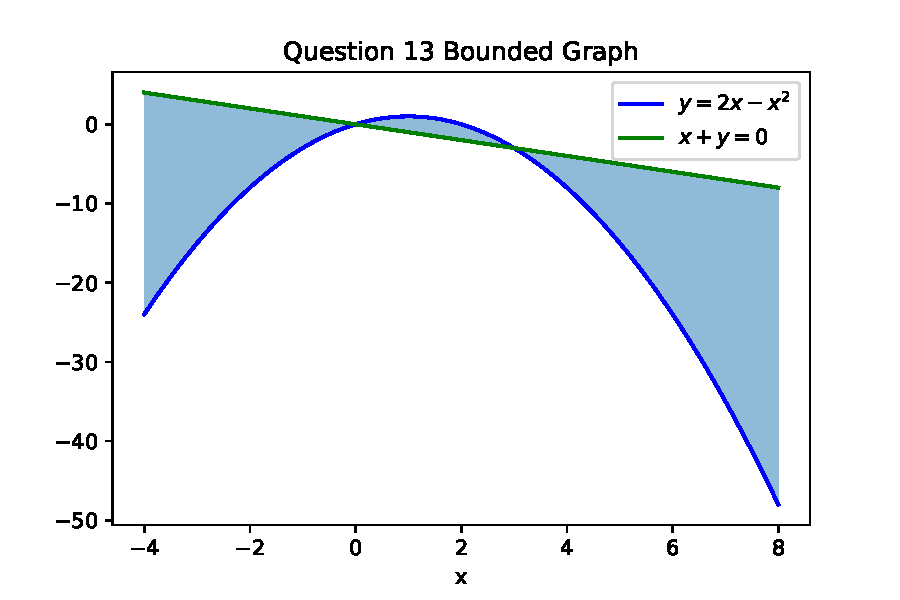
\includegraphics[width=0.4\textwidth, angle=0]{question13.pdf}


\section{Question 14}
\textbf{Solution:}

$$\int_{-2}^{2}\frac{dx}{x^3}=-\frac{1}{2}\frac{1}{x^2}\bigg|_{-2}^{2}=-\frac{1}{8}+\frac{1}{8}=0$$
Note, when the above equations exclude the point $x=0$. 














\end{document}